%%%%%%%%%%%%%%%%%%%%%%%%%%%%%%%%%%%%%%%%%%%%%%%%%%%%%%%%%%%%
%%% ELIFE ARTICLE TEMPLATE
%%%%%%%%%%%%%%%%%%%%%%%%%%%%%%%%%%%%%%%%%%%%%%%%%%%%%%%%%%%%
%%% PREAMBLE 
\documentclass[9pt,lineno]{elife}
% Use the onehalfspacing option for 1.5 line spacing
% Use the doublespacing option for 2.0 line spacing
% Please note that these options may affect formatting.

\usepackage{lipsum} % Required to insert dummy text
\usepackage[version=4]{mhchem}
\usepackage{siunitx}
\DeclareSIUnit\Molar{M}
\usepackage{indentfirst} %I prefer to have indents following section headings, I find it to be more consistent in style throughout document

\renewcommand{\floatpagefraction}{1}

%%%%%%%%%%%%%%%%%%%%%%%%%%%%%%%%%%%%%%%%%%%%%%%%%%%%%%%%%%%%
%%% ARTICLE SETUP
%%%%%%%%%%%%%%%%%%%%%%%%%%%%%%%%%%%%%%%%%%%%%%%%%%%%%%%%%%%%
\title{Transcriptional dynamics of influenza virus infection in single cells}

\author[1]{Alistair B. Russell}
\author[2]{Cole Trapnell}
\author[1,2*]{Jesse D. Bloom}
\affil[1]{Basic Sciences Division and Computational Biology Program, Fred Hutchinson Cancer Research Center, Seattle, United States}
\affil[2]{Department of Genome Sciences, University of Washington, Seattle, United States}
\corr{jbloom@fredhutch.org}{}

% \presentadd[\authfn{5}]{eLife Sciences editorial Office, eLife Sciences, Cambridge, United Kingdom}

%%%%%%%%%%%%%%%%%%%%%%%%%%%%%%%%%%%%%%%%%%%%%%%%%%%%%%%%%%%%
%%% ARTICLE START
%%%%%%%%%%%%%%%%%%%%%%%%%%%%%%%%%%%%%%%%%%%%%%%%%%%%%%%%%%%%

\begin{document}

\maketitle

\begin{abstract}
Influenza virus infection induces large changes in cellular transcription.
Previously this has mostly been looked at using bulk measurements
Here we examine the process at the level of single cells.
We find extremely wide variation in the extent of viral gene transcription across infected cells.
IFN induction is very rare.
Some cellular pathways may be consistently altered in cells with high burden of viral transcripts.
Overall, highlights remarkable heterogeneity in the outcome of infection.
\end{abstract}


\section{Introduction}

Heterogeneity is important in a lot of cellular processes even when isogenic~\citep{shalek2013single,shalek2014single}.

Population (genetic) heterogeneity is also important. 
Viral quasispecies, cancer single-cell, etc.
Salmonella paper (PhoP).

Literature on viral burst-size heterogeneity.
This goes back to Delbruck, Andino polio paper~\citep{schulte2014single}, the MDCK / flu paper.

Discuss segmented nature of influenza.
Maybe in the context of how this could further increase heterogeneity because there is a lot of potential for entire genes to be missing.
Includes Yewdell and Lowen papers.

\section{Results}

\subsection{Strategy to measure mRNA in single virus-infected cells.}
We performed single-cell mRNA sequencing using a droplet-based system that physically isolates individual cells prior to reverse transcription.
Each droplet is associated with a unique \emph{cell barcode} that tags all mRNAs from that cell during reverse-transcription.
A random \emph{unique molecular identifier (UMI)} is additionally appended to each mRNA molecule during reverse transcription.
The 3' ends of the mRNAs are sequenced and mapped to the human and influenza virus transcriptomes to determine transcript identities.
This information is combined with that provided by the UMIs and cell barcodes to quantify the number of molecules of each mRNA species that have been captured for each cell.

Infected cells will express viral as well as cellular mRNAs -- however the cell barcodes and UMIs cannot distinguish whether a cell was initially infected by one or multiple viral particles.
We therefore engineered an influenza virus (strain A/WSN/1933) that additionally carried \emph{viral barcodes} consisting of synonymous mutations near the 3' end of each transcript (Figure~\ref{fig:workflow}A).
Critically, these synonymous mutations did not greatly impact viral growth kinetics (Figure~\ref{fig:workflow}B).
We infected A549 human lung carcinoma cells with an equal mix of the wild-type and synonymously barcoded viruses.
Cells infected by a single virion will exclusively express mRNAs from either wild-type or synonymously barcoded virus, whereas cells that are co-infected with multiple virions will often express mRNAs from both the wild-type and synonymously barcoded viruses (Figure~\ref{fig:workflow}C).
\begin{figure}
\centerline{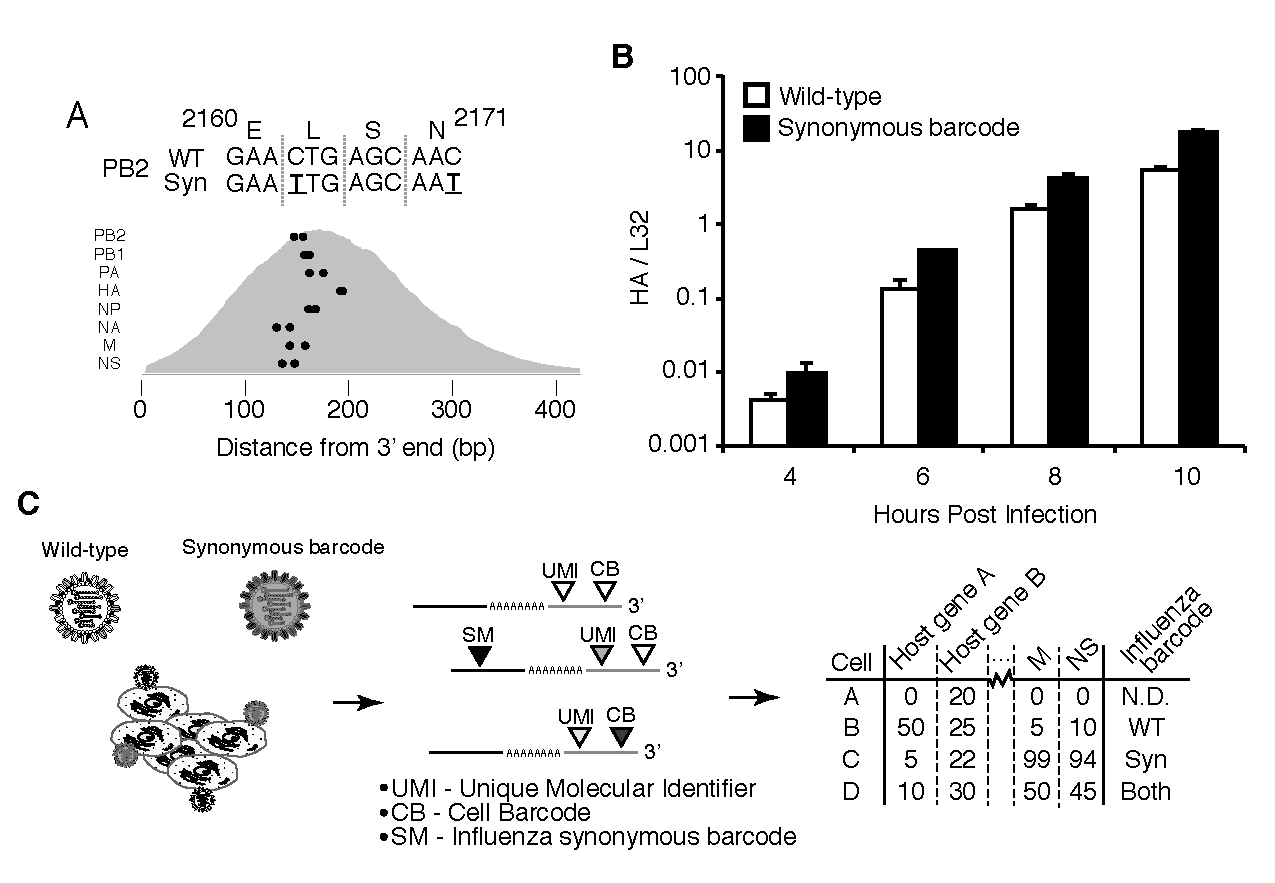
\includegraphics[width=0.8\linewidth]{figures/Workflow/workflow.pdf}}
\caption{\label{fig:workflow} Experimental design.
{\bf (A)}  
We engineered a virus that carried two synonymous mutations near the 3' end of each mRNA.
At top are the specific mutations for PB2.
At bottom are locations of the synonymous mutations relative to the typical distribution of read depth for our 3'-end sequencing.
{\bf (B)} 
The wild-type and synonymously barcoded viruses transcribe their genes with similar kinetics. 
Shown is the abundance of the viral hemagglutinin (HA) transcript relative to the cellular housekeeping gene L32 as assessed by qPCR in A549 cells infected at an MOI of 0.5 (as determined on MDCK-SIAT1 cells).
{\bf (C)}  
A549 cells were infected with an equal mixture of mutant and wild-type virus. 
Immediately prior to collection, cells were physically separated into droplets and cDNA libraries were generated containing the indicated barcodes. 
The libraries were deep sequenced, and the data processed to create a matrix that gives the number of molecules of each transcript observed in each cell.
Infected cells were further annotated by whether their viral mRNAs derived from wild-type virus, synonymously barcoded virus, or both.
}
\figdata{Sequences of wild-type and barcoded viruses are in \texttt{viralsequences.fasta}.}
\end{figure}

We took care to generate stocks of virus that were relatively ``pure'' of defective particles.
Stocks of viruses typically contain an array of biologically active viral particles, some of which are defective for replication owing to mutations or deletions in essential viral genes.
These defective particles become prevalent when a virus is grown at high multiplicity of infection (MOI), where complementation permits the growth of otherwise deleterious genotypes.
To minimize the levels of defective particles, we propagated our viral stocks at low MOI for a relatively brief period of time~\citep{xue2016propagation}.
We then validated that our stocks exhibited greater purity of infectious particles than a stock propagated at high MOI by verifying that they had a higher ratio of infectious particles to both virion RNA (Figure~\ref{fig:viruspopulations}A) and particles capable of inducing expression of a single viral protein (Figure~\ref{fig:viruspopulations}B).
In addition, viral stocks with many defective particles are more immunostimulatory~\citep{tapia2013defective}.
We confirmed that our viral stocks induced much less interferon than a stock propagated at higher MOI (Figure~\ref{fig:viruspopulations}C).

\begin{figure}
\centerline{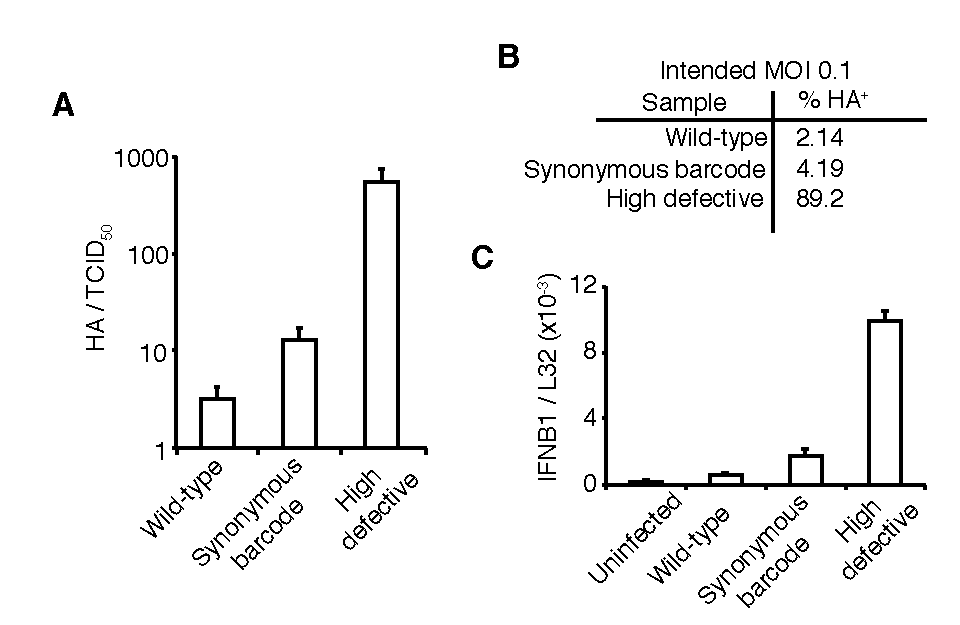
\includegraphics[width=0.7\linewidth]{figures/Validating_barcode_virus/validating_populations_D02.pdf}}
\caption{\label{fig:viruspopulations} The viral stocks in our experiments are relatively pure of defective particles. 
{\bf (A)}
Our viral stocks have a higher ratio of infectious particles to HA virion RNA compared to a high-defective stock propagated at high MOI.
HA viral RNA was quantified by qPCR on virions. 
{\bf (B)} 
Our viral stocks have a higher ratio of infectious particles to particles capable of expressing the viral HA protein.
A549 cells were infected with all three viral stocks at an MOI of 0.1, and the percentage of cells expressing HA protein at 9 hours post-infection was quantified by antibody staining and flow cytometry.
{\bf (C)} 
Our viral stocks are less immunostimulatory than virus propagated at high MOI. 
Measurements of \textit{IFNB1} transcript by qPCR normalized to the housekeeping gene L32 in A549 cells at 10 hours post infection at an MOI of 0.5.
MOIs were calculated by TCID50 on MDCK-SIAT1 cells.}
\figsupp[Flow cytometry data for calculating the percentage of HA-expressing cells.]{Longer caption}{\emph{HA-expression flow cytometry supplemental figure needs to be created.}}
\end{figure}

\subsection{Single cells show a wide range of expression of viral transcripts.}
We infected A549 cells at low MOI with a mixture of the wild-type and synonymously barcoded viruses, and collected cells for sequencing at 6, 8, and 10 hours post-infection, including a replicate of the 8-hour timepoint.
We recovered between 3,000 and 4,000 cells for each sample (Figure~\ref{fig:cells}A). 
As expected for a low-MOI infection, most cells expressed little or no viral mRNA (Figure~\ref{fig:cells}B).
Also as expected, the amount of viral mRNA per cell among infected cells increased over time (Figure~\ref{fig:cells}B).
But what was most notable was how widely the number of viral mRNA molecules varied among infected cells.
While the fraction of mRNA derived from virus was $<$0.1\% for most cells, viral mRNA constituted close to half the transcriptome in a few cells at 8 and 10 hours (Figure~\ref{fig:cells}C).
%Therefore, there is extraordinary variability in the number of viral transcripts per infected cell.

\begin{figure}
\centerline{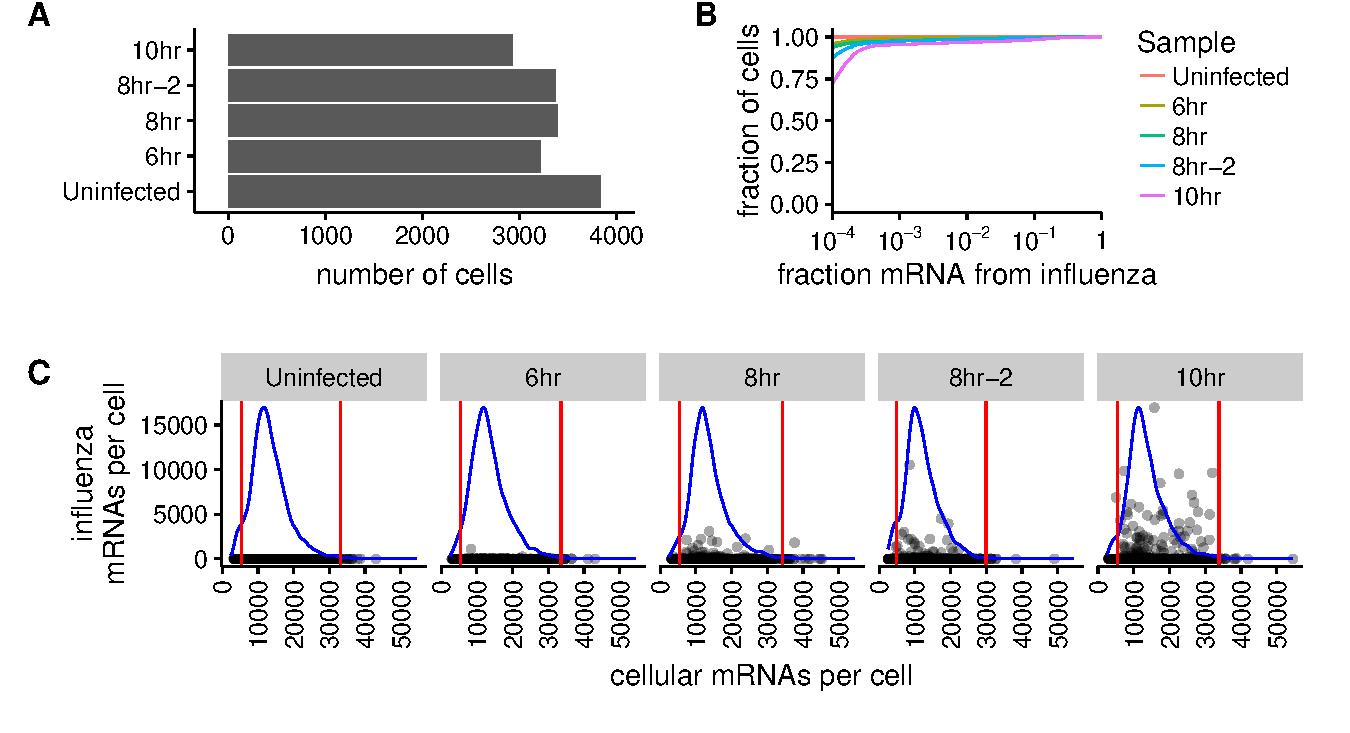
\includegraphics[width=0.9\linewidth]{figures/p_cell_mRNA_summary.pdf}}
\caption{\label{fig:cells}
There is a very wide distribution in the number of viral mRNAs detected per cell.
{\bf (A)} 
Number of cells sequenced for each sample.
{\bf (B)} 
Cumulative distribution of the fraction of mRNA derived from influenza virus for each sample.
For each point on the x-axis, the y-axis indicates the fraction of cells with at least that much of their mRNA from virus.
{\bf (C)} 
The number of cellular and viral mRNAs for each cell is plotted as a point.
The blue lines show the overall distribution of the number of cellular mRNAs per cell.
Cells outside the red lines were considered outliers (possibly derived from two cells per droplet), and were excluded from subsequent analyses.
}
\end{figure}

A complicating factor is that uninfected cells could have small amounts of viral mRNA due to leakage of transcripts from lysed cells.
It is therefore important to establish a threshold for identifying truly infected cells.
We can do this by taking advantage of the fact that roughly half the infecting virions bear synonymous barcodes.
Reads derived from lysed cells will be drawn from both wild-type and synonymously barcoded viral transcripts.
However, most cells are infected by at most one virion, and so the reads from truly infected cells will usually derive almost entirely from one of the two viral variants. 
Figure~\ref{fig:viralbarcodes}A shows the fraction of viral reads in individual cells from each viral variant, and Figure~\ref{fig:viralbarcodes}B indicates the fraction of viral reads from the most abundant variant in that cell.
Most cells with large amounts of viral mRNA have viral transcripts exclusively derived from one viral variant -- indicating non-random partitioning as expected from viral infection.
However, cells with a small amount of viral mRNA often have viral transcripts from both variants, as expected from the random partitioning associated with simple mRNA leakage.
Finally, a few cells with large amounts of viral mRNA have viral transcripts from both variants, reflecting co-infection with both variants.

We determined the threshold amount of viral mRNA per cell at which the barcode partitioning clearly resulted from infection rather than leakage (Figure~\ref{fig:viralbarcodes}C), and used this threshold to annotate cells that we were confident were truly infected.
We also annotated as co-infected cells above this threshold that had mRNA from both viral variants.
Figure~\ref{fig:viralbarcodes}D shows the number of cells annotated as infected and co-infected for each sample -- these cells are just a small fraction of the number of cells with any viral read.
These annotation thresholds are conservative, and will miss some true low-level infections, as well as any co-infections with the same viral variant.
However, it is important that the analyses below are restricted to cells that are truly infected with virus, so we accepted the loss of some low-level infections in order to avoid false positives.
Because the bulk of cells are not infected, we subsampled the uninfected cells to the numbers shown in Figure~\ref{fig:viralbarcodes}D to balance the proportions of infected and uninfected cells for all subsequent analyses.

Strikingly, the extreme variation in the number of viral transcripts per cell remains even after we apply these rigorous criteria for annotating infected cells (Figure~\ref{fig:viralbarcodes}E). 
The fraction of viral mRNA per infected cell follows a roughly exponential distribution, with many cells having few viral transcripts and a few cells having many.
In fact, a bare few infected cells contribute the majority of influenza transcripts.
Specifically, at 6 and 8 hours $<$10\% of infected cells are responsible for over half the viral transcripts, while at 10 hours $\approx$15\% of infected cells produce over half the viral transcripts (Figure~\ref{fig:viralbarcodes}-Figure~supplement~\ref{figsupp:cumulfracflu}).

\begin{figure}[t!]
\centerline{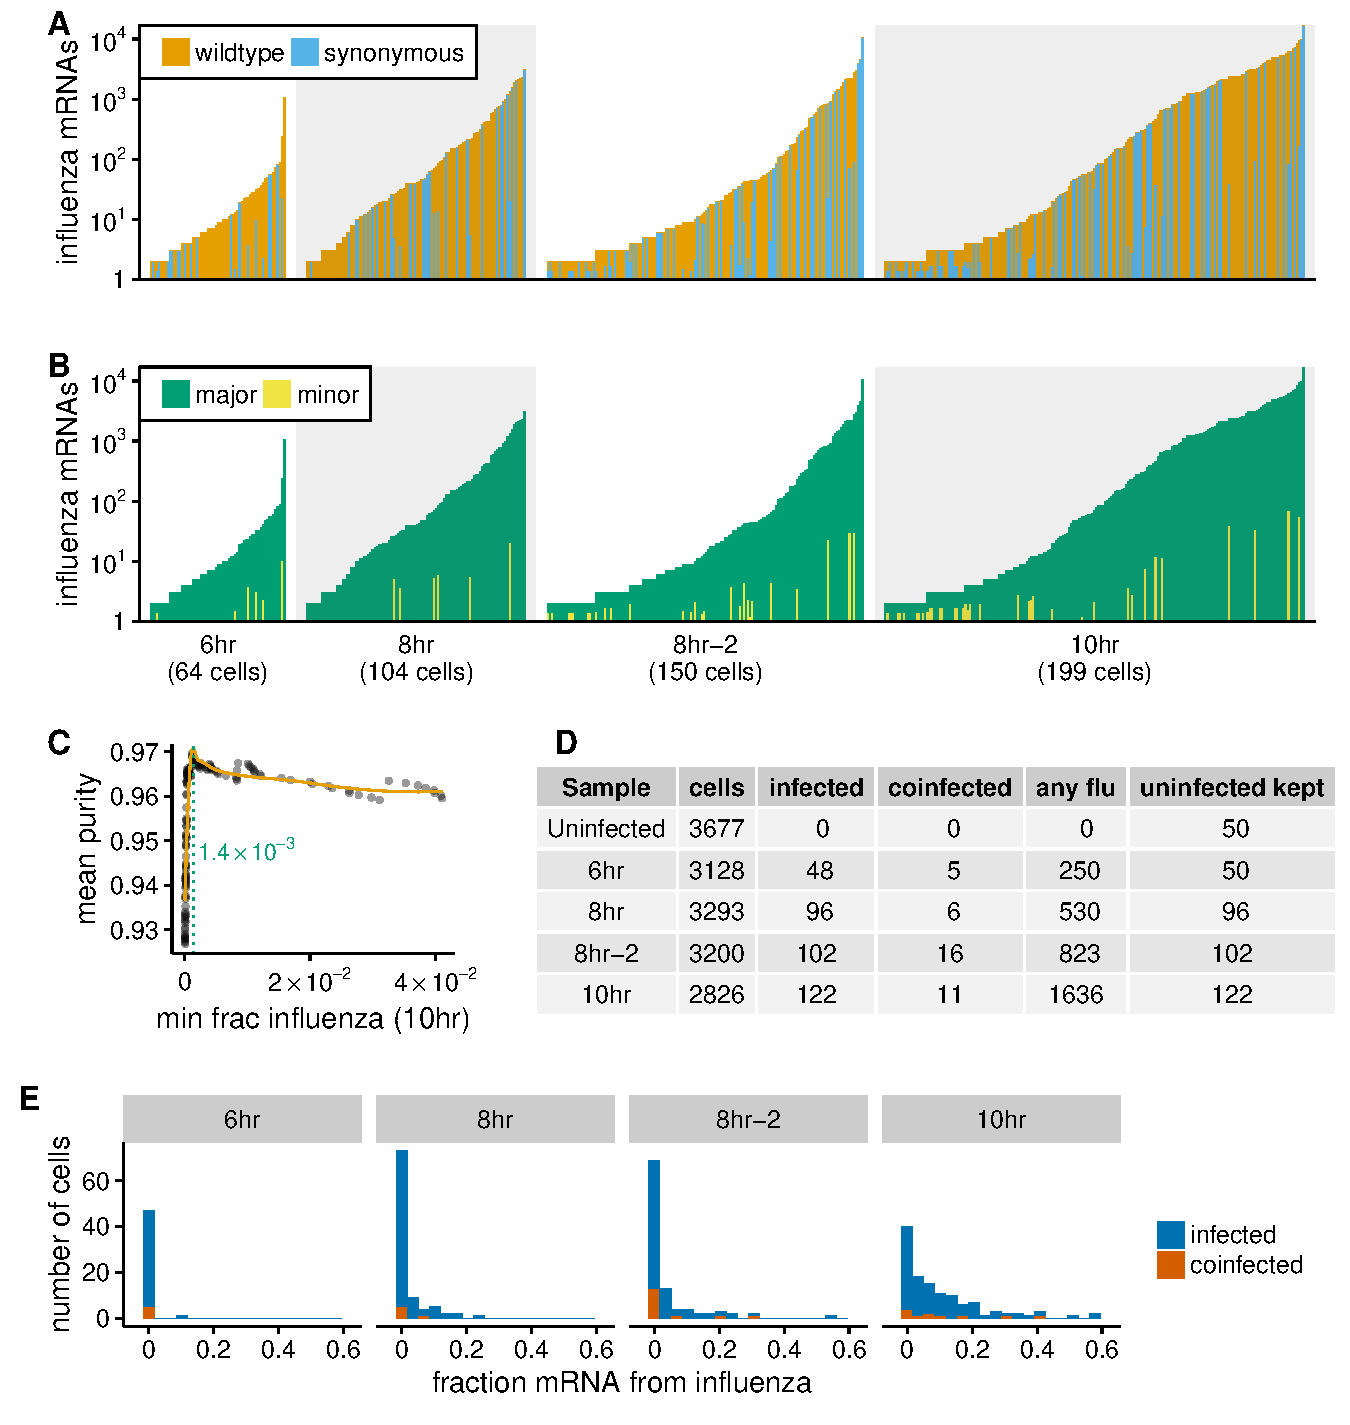
\includegraphics[width=0.9\linewidth]{figures/p_frac_flu_summary.pdf}}
\caption{\label{fig:viralbarcodes}
Synonymous barcodes on the viral mRNAs distinguish true infections from cells that contain viral mRNAs derived from leakage of lysed cells.
{\bf (A)}
Cells with at least two viral mRNAs for which the barcode could be called, arranged in order of increasing influenza transcript counts.
Bar heights denote the number viral mRNAs on a log\textsubscript{10} scale, bar coloring is linearly proportional to the fractions of viral mRNAs derived from wild-type and synonymously barcoded virus.
{\bf (B)}
Same as (A), but each bar is colored according to the relative fraction of the more common (major) and less common (minor) virus variant.
At low levels of viral mRNA there is often a roughly equal mix, suggesting contamination with viral mRNAs leaked from lysed cells.
At higher levels of viral mRNA, cells generally have only one viral variant, suggesting infection initiated by a single particle.
A few cells are also obviously co-infected with both viral variants.
{\bf (C)}
We determined a cutoff for calling ``true'' infections by fitting a curve to the mean barcode purity of all cells with greater than a given fraction of their mRNA derived from virus.
We called the cutoff at the point at which purity stops increasing with the fraction of viral mRNA.
{\bf (D)}
The number of cells identified as infected and co-infected for each sample, as well as the number of cells with any viral read.
For all subsequent analyses, we subsampled the number of uninfected cells per sample to the greater of 50 or the number of infected cells.
{\bf (E)} 
Distribution of the fraction of mRNA per cell derived from virus for both infected and co-infected cells.
}
\figsupp[Number of viral barcodes called.\label{figsupp:barcodescalled}]{
The number of viral barcodes called for each sample and influenza gene segment. 
Viral transcripts are classified as \emph{syn} if they mapped to a synonymously barcoded influenza transcript, \emph{wt} if they mapped to a wild-type influenza transcript, \emph{invalid} if multiple reads for the same UMI differed on the status of the viral barcode, and as \emph{uncalled} if none of the reads for that UMI overlapped the region of the viral transcript containing the viral barcode.
}{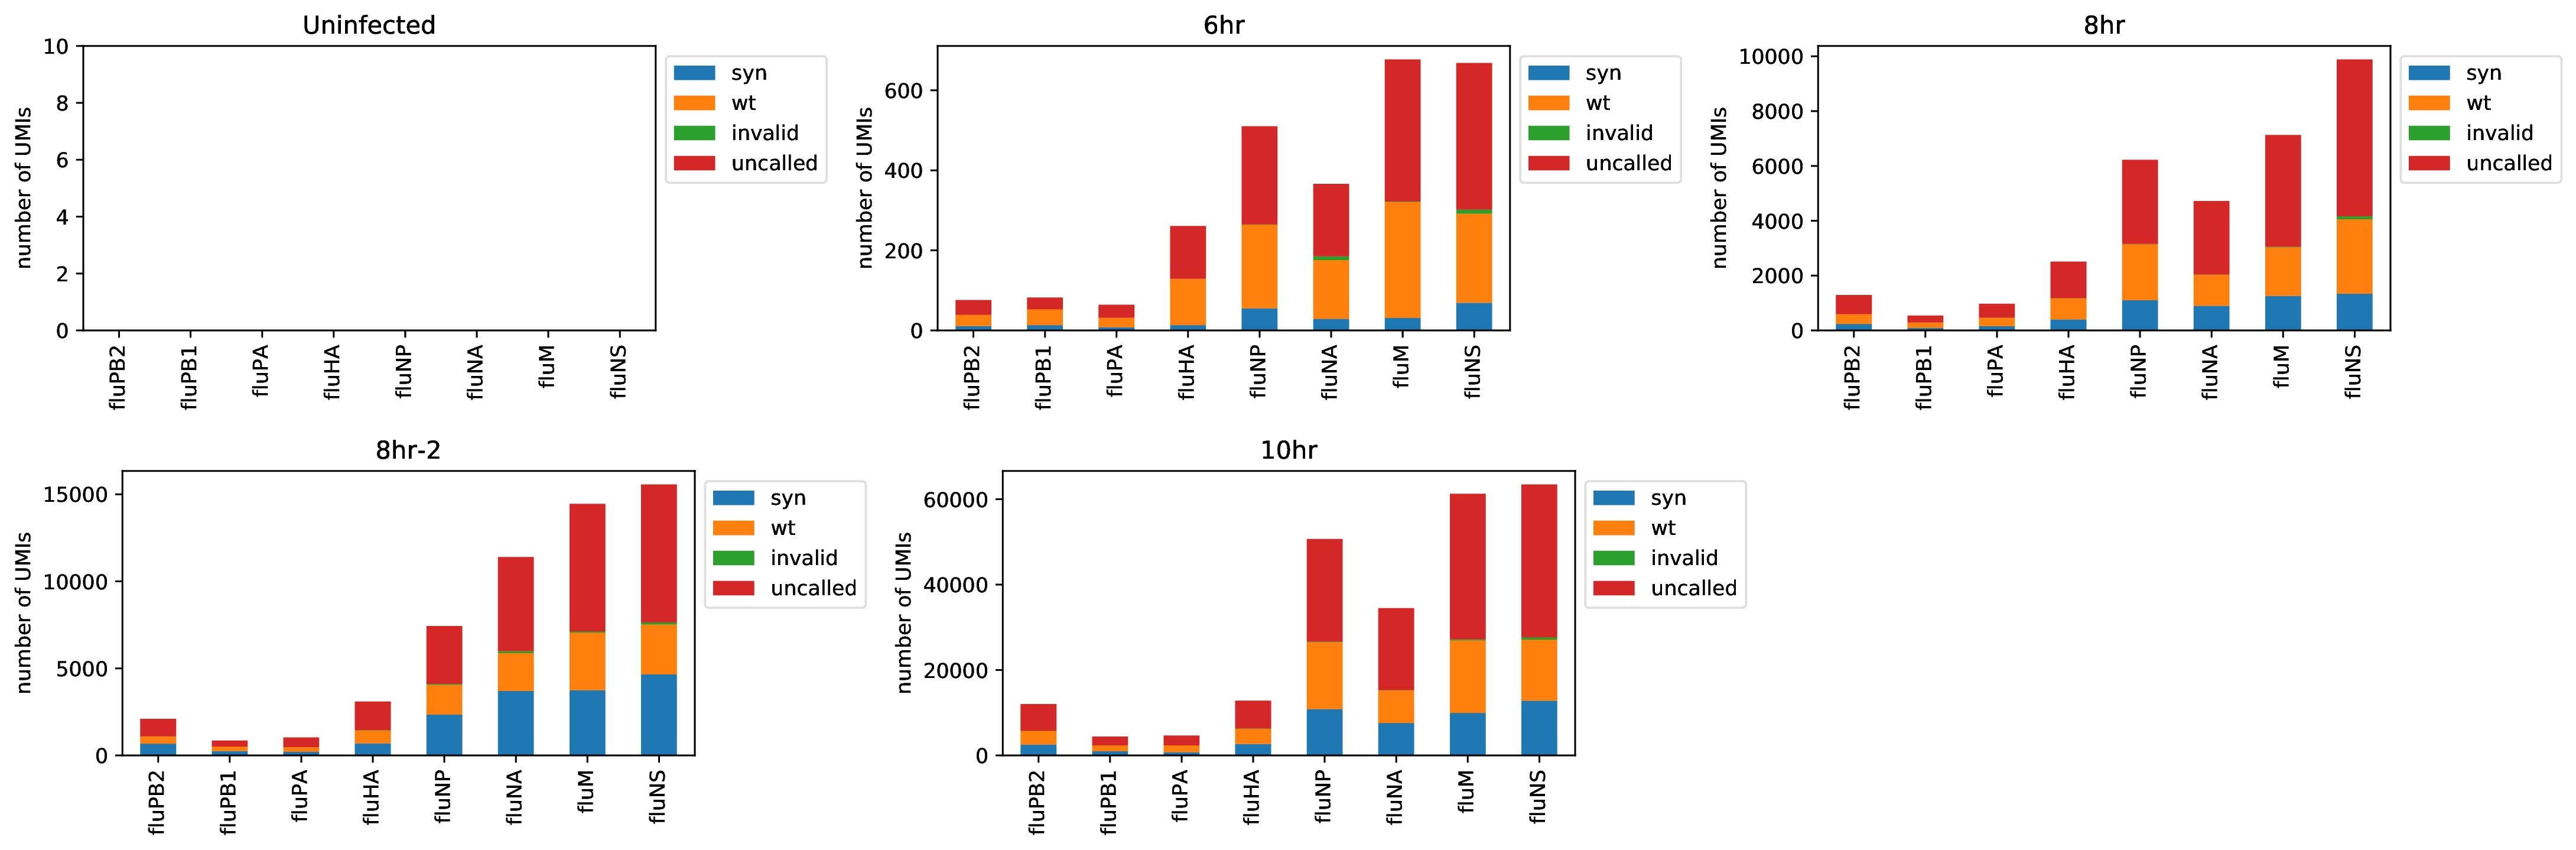
\includegraphics[width=\linewidth]{figures/synbarcodes_umistats.jpg}}
\figsupp[Fraction of total viral mRNA derived from a given fraction of infected cells.\label{figsupp:cumulfracflu}]{
The total fraction of all viral mRNA among infected cells that is attributable to a given fraction of these cells.
For instance, the plot for the 8-hour sample shows that roughly 50\% of all viral mRNA is derived from 10\% of the infected cells.
}{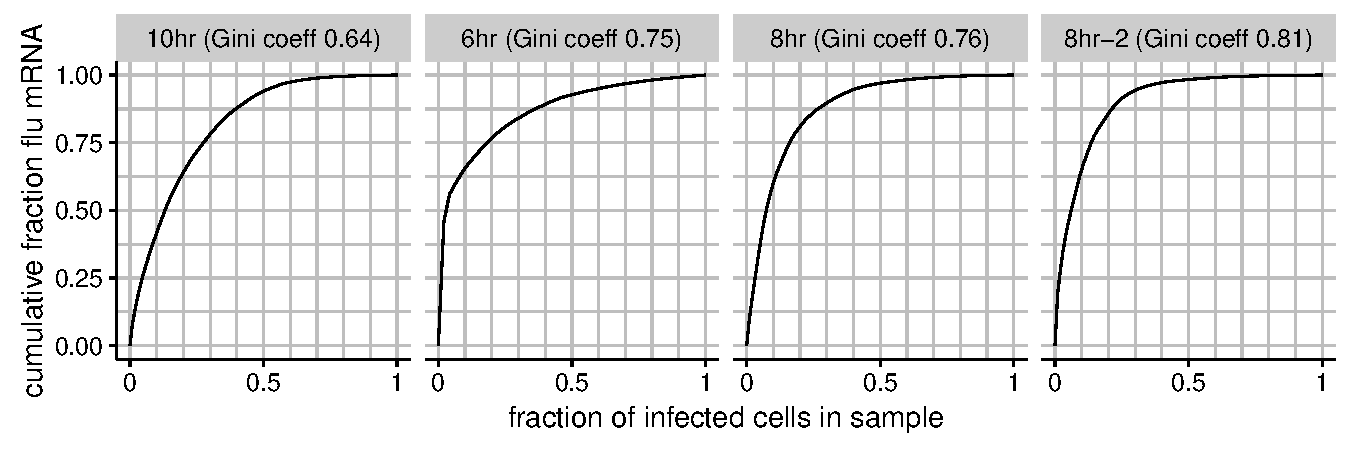
\includegraphics[width=\linewidth]{figures/p_cumul_flu.pdf}}
\end{figure}

\subsection{Absence of viral genes partially explains cell-to-cell variability in viral transcript abundance.}
The influenza genome is segmented, and cells can fail to express a viral mRNA if the encoding gene segment is not packaged in the infecting virion or fails to initiate transcription after infection.
Indeed, several groups have reported that the majority of infected cells fail to express at least one viral gene~\citep{brooke2013most}. 
We wondered if the absence of specific viral genes might be associated with reduced amounts of viral mRNA within single infected cells.
In particular, transcription of influenza virus mRNAs is performed by the viral ribonucleoprotein (RNP) complex, which consists of the three proteins that encode the tripartite polymerase (PB2, PB1, and PA) as well as nucleoprotein (NP).
Each viral gene segment is associated with one RNP in incoming infecting virions, but secondary transcription by newly synthesized RNPs requires the presence of the viral genes for each of the four constituent RNP proteins so that the cell can produce more RNP proteins.
This secondary transcription is a major source of viral mRNAs, as evidenced by the fact that blocking synthesis of the RNP proteins reduces the amount of viral mRNA by several orders of magnitude in bulk cells (Figure~\ref{fig:fluburdenbyflugene}-Figure~supplement~\ref{figsupp:cyclohexamide}).

\begin{figure}[t!]
\centerline{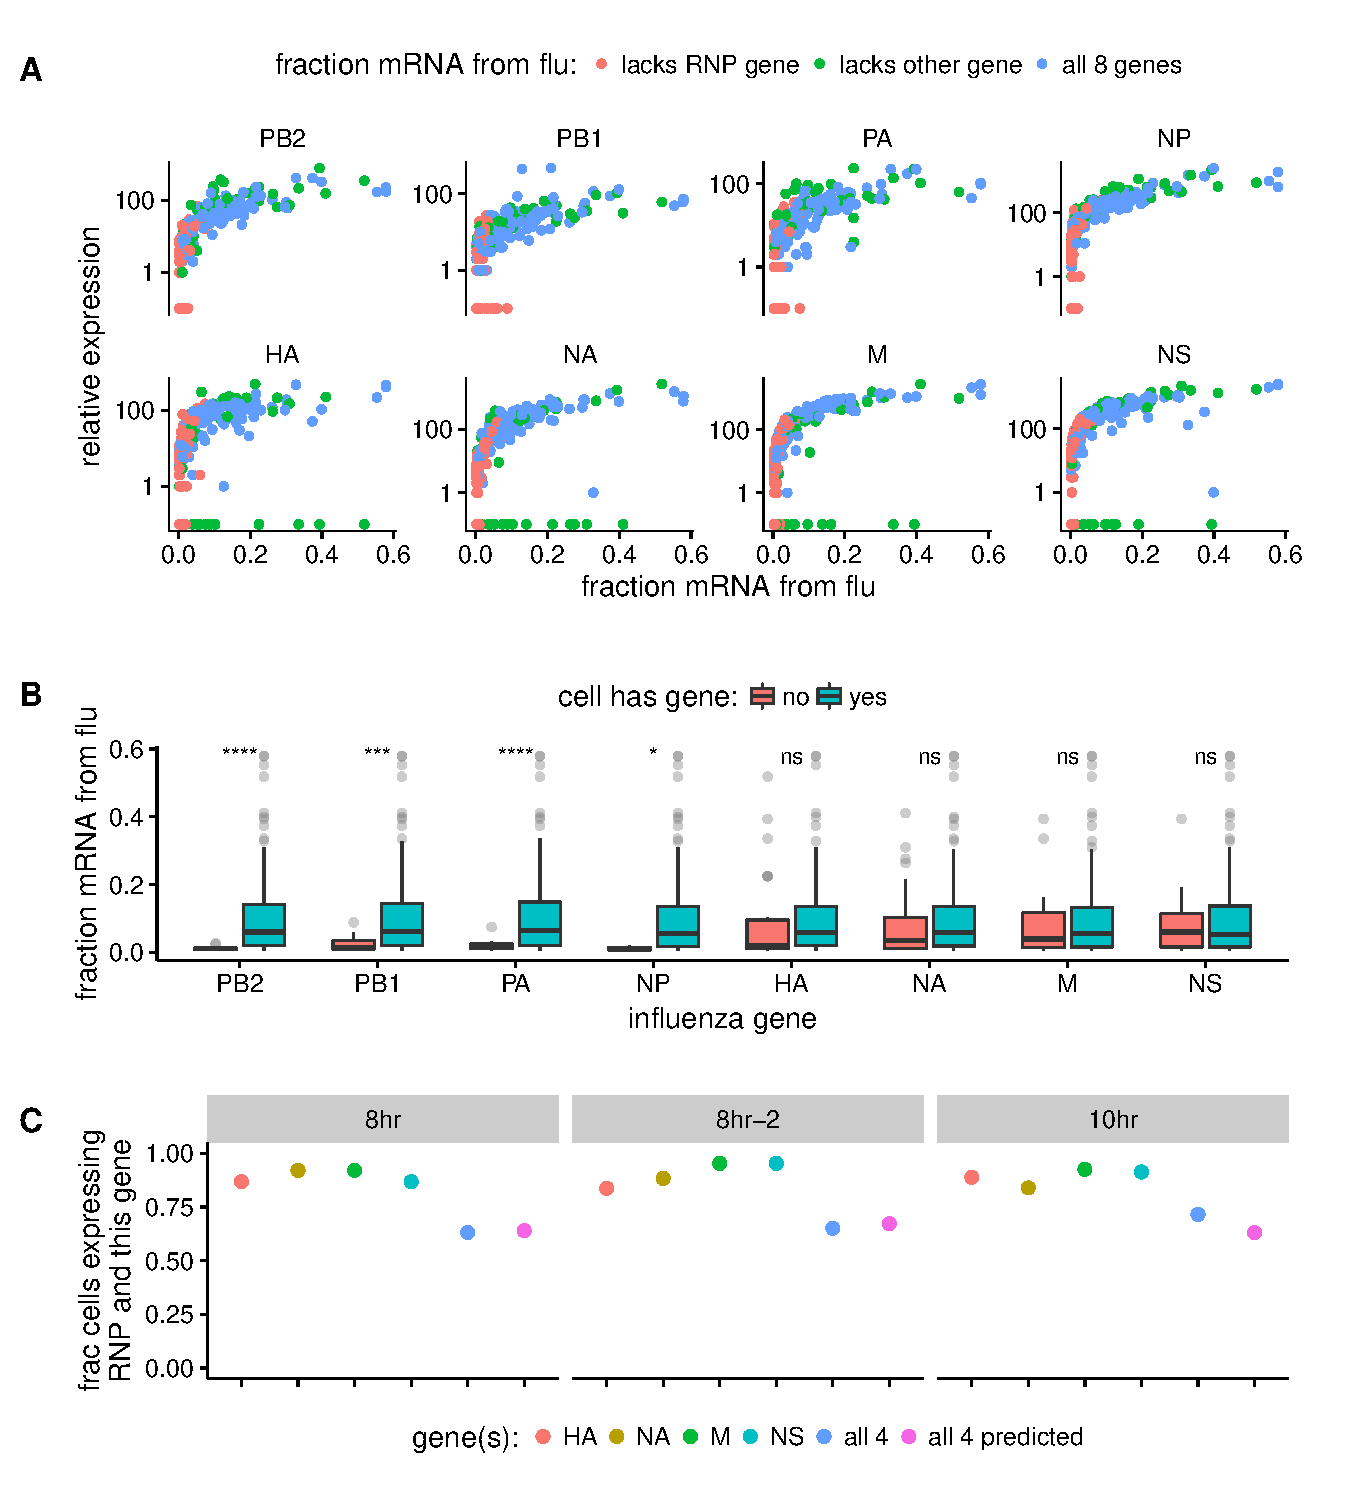
\includegraphics[width=0.9\linewidth]{figures/p_flu_burden_flu_gene_merge.pdf}}
\caption{\label{fig:fluburdenbyflugene}
The absence of viral genes explains some of the variability in the amount of viral mRNA per cell.
{\bf (A)} 
Fraction of mRNA in each infected cell derived from virus as a function of the normalized expression of each viral gene in that cell, taken over all time points.
Cells with high viral burden always express all the RNP genes, but some cells with high viral burden lack each of the other viral genes.
{\bf (B)}
Box plots showing the per-cell viral burden among cells with $>$0.5\% of their mRNA from virus, binned by whether or not the cells express each viral gene.
A Wilcoxon signed-rank test was used to test the null hypothesis that absence of each gene does not affect viral burden: **** = $P < 10^{-4}$, *** = $P < 10^{-3}$,  * = $P < 0.05$.
Similar results are obtained if we examine only the 10-hour timepoint (Figure~\ref{fig:fluburdenbyflugene}-Figure~supplement~\ref{figsupp:10hrfluburdenbyflugene}).
{\bf (C)}
Fraction of infected cells that express all four RNP genes and also express each of the four other genes, as well as the fraction that express \emph{all} four of the other genes.
The fraction of cells that express all four other genes is well predicted by simply multiplying the frequencies of cells that express each of these genes individually, indicating that gene absence is approximately independent across these four genes.
}
\figsupp[Secondary transcription from newly synthesized RNPs is a major source of viral mRNA during bulk infections.\label{figsupp:cyclohexamide}]{
A549 cells were infected at an MOI of 0.2 as calculated on MDCK-SIAT1 cels in either the presence or absence of the protein-translation inhibitor cyclohexamide, and viral mRNA was quantified at 8 hours post-infection by qPCR.
The cyclohexamide prevents translation of new PB2, PB1, PA, and NP protein, and so prevents the formation of the new RNPs needed for secondary transcription.
The bars show the relative amount of HA and PB2 mRNA in the absence versus the presence of cyclohexamide.
}{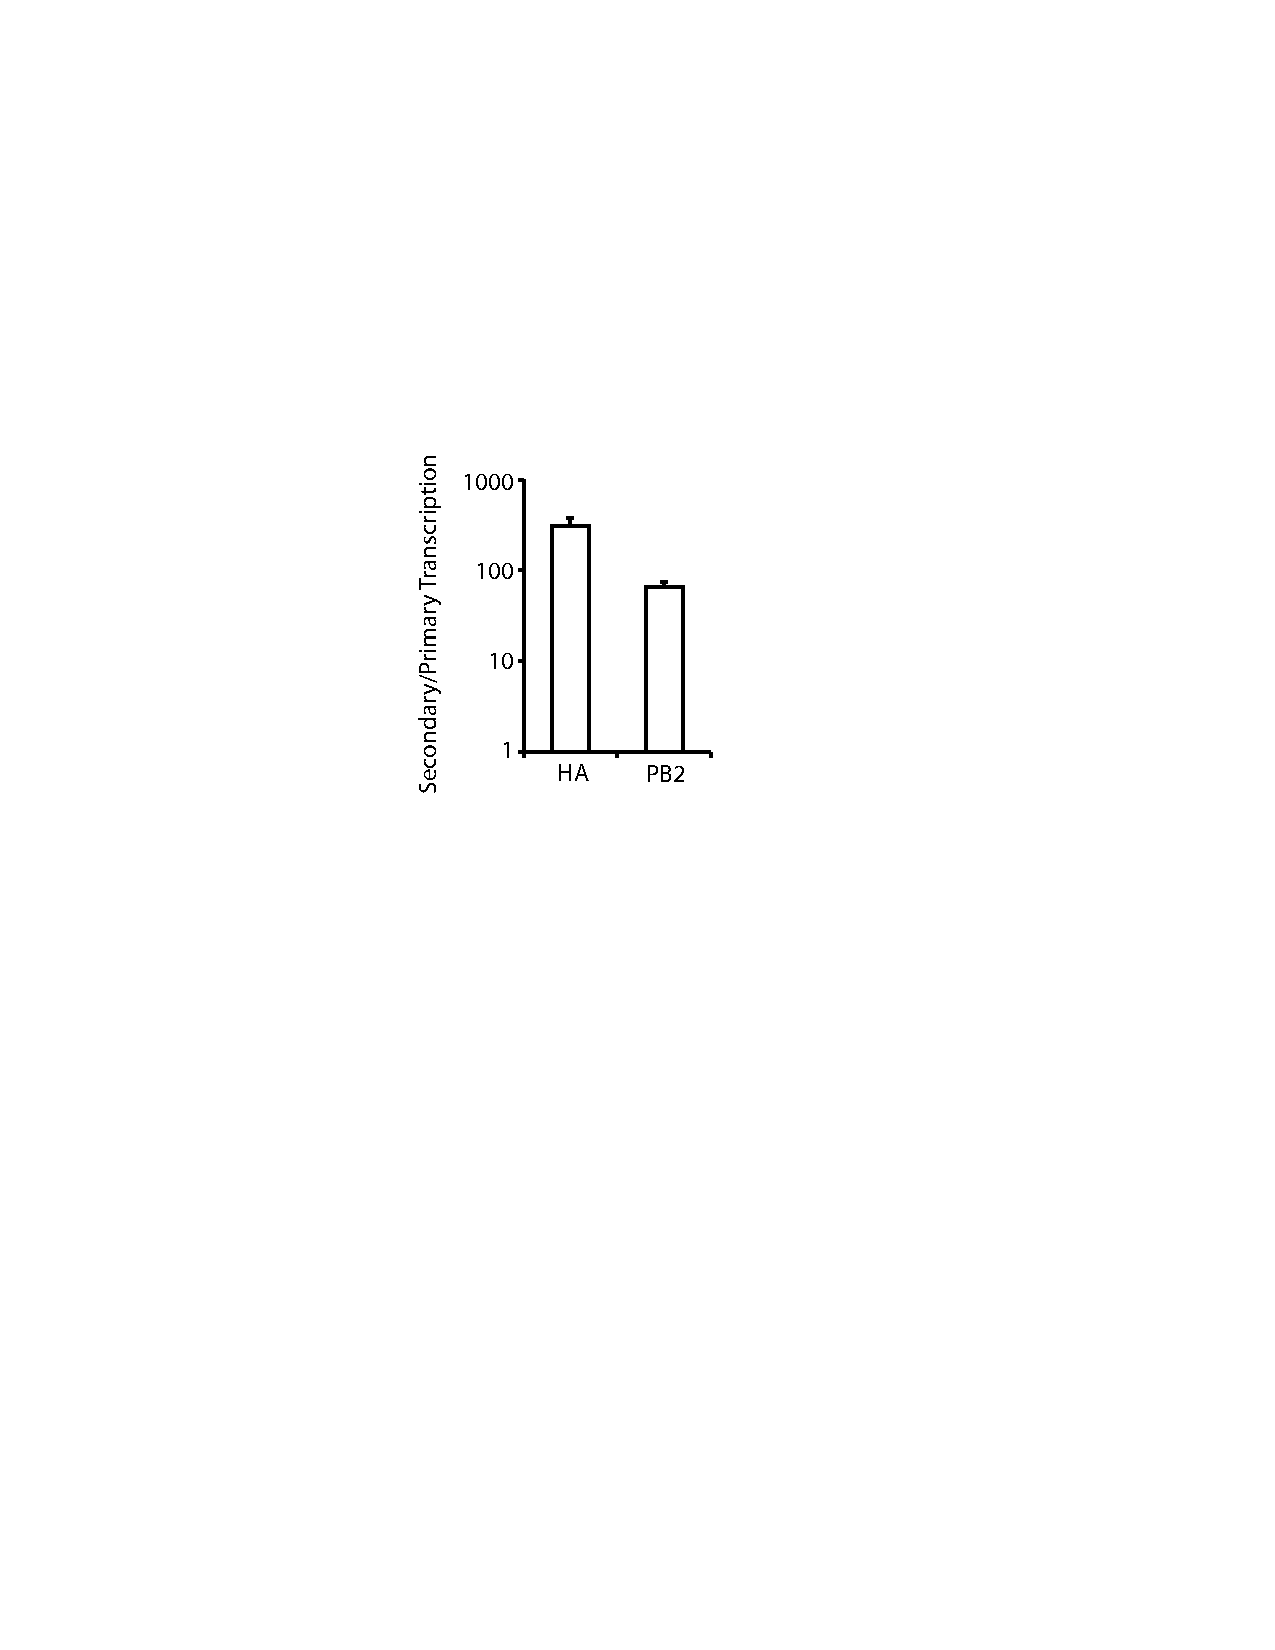
\includegraphics[width=0.3\linewidth]{figures/Primary_transcription_measurements/Cyclohexamide.pdf}}
\figsupp[Like panel (B) but for the 10-hr sample only.\label{figsupp:10hrfluburdenbyflugene}]{
The absence of viral RNP genes but \emph{not} non-RNP genes remains significantly associated with reduced viral burden when we examine only the 10-hr sample, which is the single time point with the most data points.
The difference for NP is no longer statistically significant due to low counts of infected cells lacking NP, but the trend remains.
}{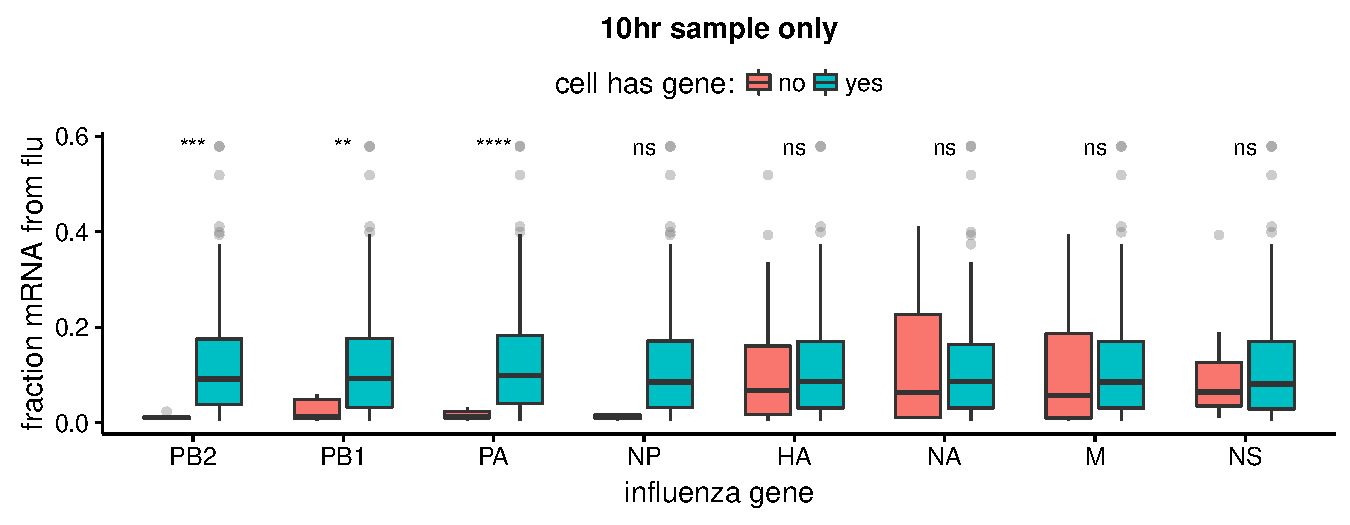
\includegraphics[width=\linewidth]{figures/p_10hr_flu_burden_flu_gene_test}}
\figdata{The numerical data for panel (C) are in \texttt{p\_missing\_genes.csv}.}
\end{figure}

We examined the total fraction of mRNA in each cell that derives from virus versus the relative expression of each viral gene (Figure~\ref{fig:fluburdenbyflugene}A). 
Cells that lack an RNP gene never derive more than a few percent of their mRNAs from virus, demonstrating that the presence of these RNP genes is essential for high levels of viral transcription.
However, we observe cells that lack each of the other non-RNP genes but still derive $\approx$40\% of their mRNAs from virus, suggesting that none of the other genes are important for high levels of viral transcription.
These results are statistically supported by Figure~\ref{fig:fluburdenbyflugene}B, which shows that absence of any RNP gene but \emph{not} any of the other viral genes is associated with reduced amounts of viral mRNA. 
However, gene absence clearly does not explain all of the variability in viral gene expression, since even cells expressing all viral genes exhibit a very wide distribution in the amount of viral mRNA that they express. 
The rest of this variability must be due to additional mechanisms such as differences in host-cell state, viral mutations not detectable by our 3'-end sequencing approach, or inherent stochasticity.  

We also sought to quantify the fraction of infected cells that completely failed to express a given gene.
We limited this analysis to examining the presence / absence of the non-RNP genes in cells expressing all four RNP genes, since we might fail to detect viral transcripts that are actually present at low levels in RNP-deficient cells due to the lower viral burden in these cells.
At the 8- and 10-hour time points, between 5\% and 17\% of cells fail to express any one of the four non-RNP genes (Figure~\ref{fig:fluburdenbyflugene}C).
The absence of a given gene appears to be an independent event, as the probability of observing all four non-RNP genes in a cell is well predicted by simply multiplying the probabilities of observing each gene individually (Figure~\ref{fig:fluburdenbyflugene}C). 
Our measurements of the frequency at which infected cells fail to express individual viral genes are roughly consistent with estimates made by others using different means~\citep{brooke2013most}.
	
\subsection{The relative amounts of different viral mRNAs are fairly consistent across cells.}
The results above show that the total amount of viral mRNA in infected cells varies over orders of magnitude.
Does the relative expression of viral genes exhibit similar cell-to-cell variability?
To address this question, we focused on cells that derived $>$5\% of their mRNA from virus, since estimates of relative viral gene expression will be less noisy in cells with more viral mRNAs.

\begin{figure}
\centerline{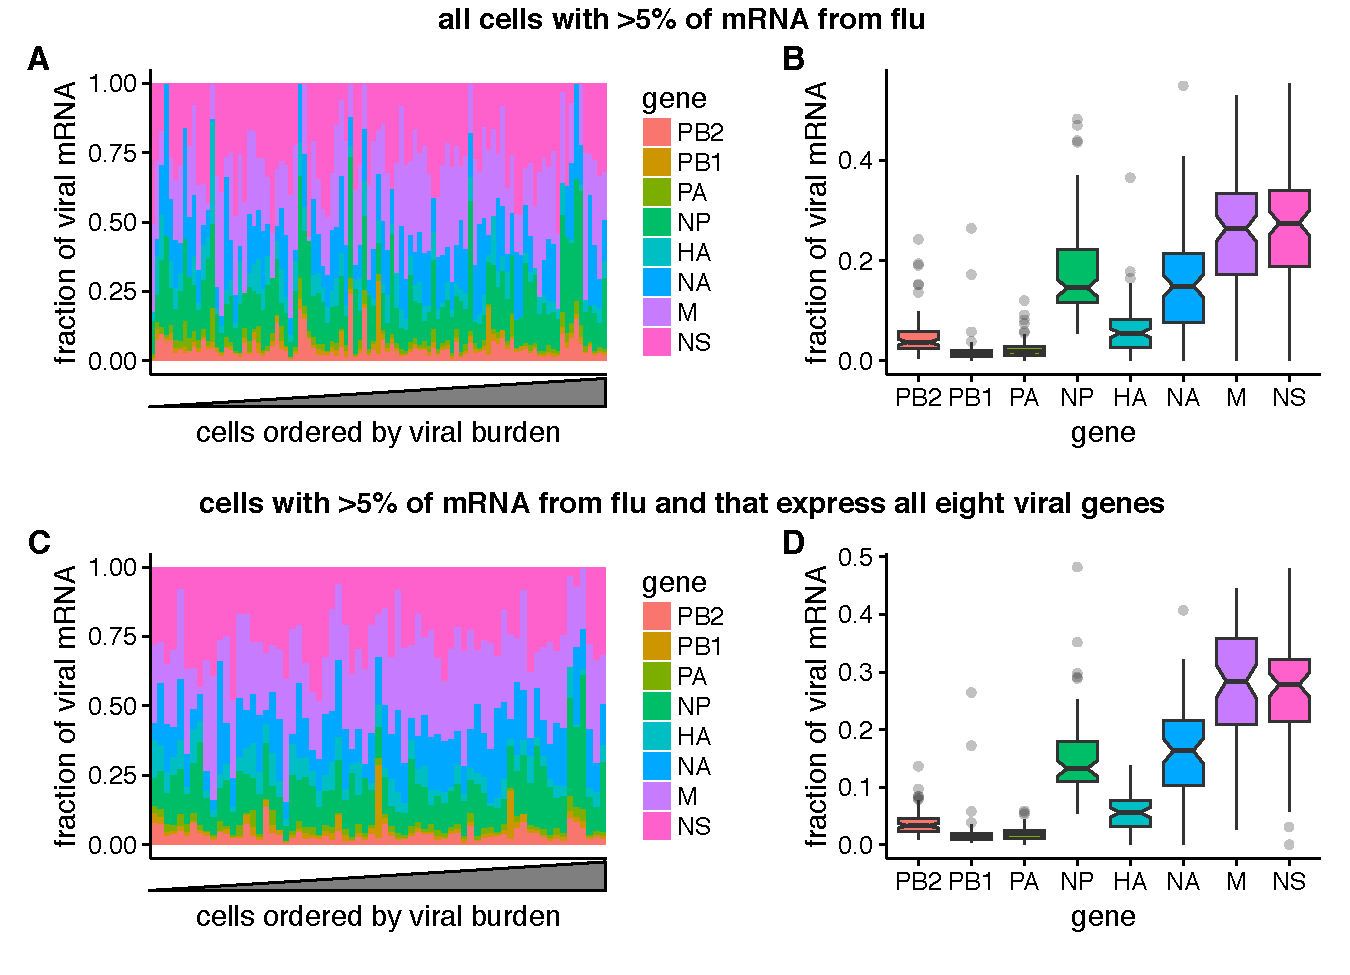
\includegraphics[width=0.9\linewidth]{figures/p_flu_expr_aledit.pdf}}
\caption{\label{fig:fluexpr}
Relative expression of influenza virus genes in highly infected cells (>5\% of total mRNA from virus).
{\bf (A)} 
The fraction of viral mRNA from each viral gene for each cell. 
{\bf (B)}
Box plots showing the distribution of the fraction of viral mRNA per cell from each viral gene.
The black lines at the notches are the medians, and the tops and bottoms of boxes indicate the first and third quartiles.
{\bf (C)}, {\bf (D)} 
The same plots, but only including cells for which we observed at least one molecule of each viral gene.
}
\figdata{The raw data are in \texttt{p\_flu\_expr.csv}.}
\end{figure}

In contrast to the extreme variability in the total viral mRNA per cell, the fraction of this mRNA derived from each gene is much more consistent across cells (Figure~\ref{fig:fluexpr}A).
Total viral mRNA varies by orders of magnitude, but the fraction from any given viral gene is fairly tightly clustered around the median value for all cells (Figure~\ref{fig:fluexpr}B).
The relative levels of each viral mRNA in our cells are similar to prior bulk measurements made by Northern blots~\citep{hatada1989control}, which also found an expression hierarchy of M $>$ NS $\gg$ NP $>$ NA $>$ HA $\gg$ PB2 $\sim$ PB1 $\sim$ PA.
The cell-to-cell consistency in the relative expression of different viral genes generally becomes even tighter if we limit the analysis only to cells that express all eight viral genes (Figure~\ref{fig:fluexpr}C,D).
Therefore, with the exception of complete gene absence, the factors that drive the dramatic cell-to-cell variability in the amount of viral mRNA appear to have roughly similar effects on all viral genes in a given cell.
This finding is consistent with prior work showing positive correlations among the abundance of several viral gene segments in individual cells.

\subsection{Co-infection can provide infected cells with the full complement of viral genes.}
Our sequencing enables us to identify the rare cells that were co-infected with both wild-type and synonymously barcoded viral variants.
Overall, we captured 10 such co-infected cells that had $>$5\% of their mRNA derived from virus (Figure~\ref{fig:coexpression}).
Seven of these 10 cells expressed all eight viral genes.
Remarkably, the majority (4 of 7) of these cells would \emph{not} have expressed all the viral genes in the absence of co-infection, since they have at least one gene exclusively derived from each viral variant.
For instance, the cell with 11.2\% of its mRNA from virus in the upper right of Figure~\ref{fig:coexpression} expresses M only from the wildtype viral variant, and NP and HA only from the synonymously barcoded variant.
Our data therefore provide direct single-cell support for the idea that co-infection can rescue missing viral genes~\citep{brooke2013most}.

\begin{figure}
\centerline{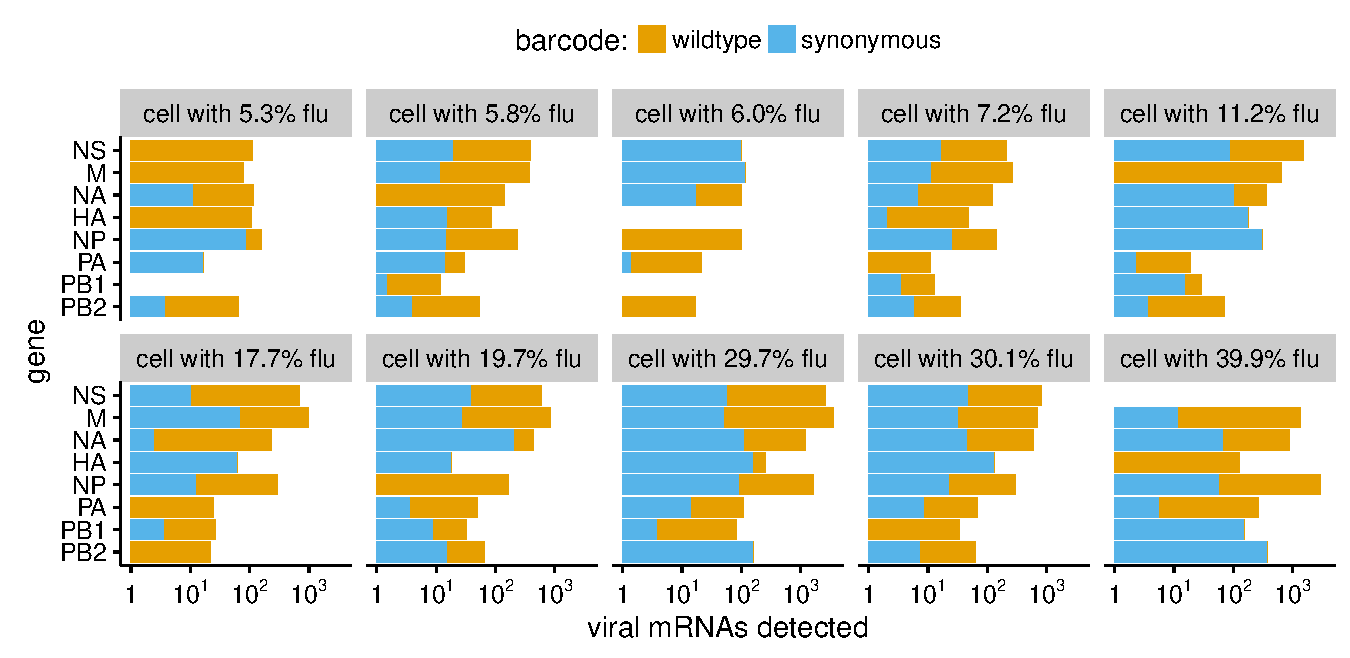
\includegraphics[width=0.9\linewidth]{figures/p_coinfection.pdf}}
\caption{\label{fig:coexpression}
The abundance of each viral transcript in cells that are co-infected with the two viral variants and have $>$5\% of their mRNA derived from virus.
The bars show the logarithm of the numbers of each viral mRNA detected, and are colored in linear proportion to the fraction of that mRNAs derived from wild-type or synonymously barcoded virus.
}
\figsupp[Co-infected cells express roughly equal amounts of a gene from each infecting viral variant. \label{figsupp:flowcyto}]{
{\bf(A)} Cells were co-infected with a mix of wild-type virus and virus in which the HA gene was replaced by GFP flanked by the terminal regions of the HA gene segment. 
At 10 hours post-infection, cells were analyzed by flow cytometry for HA and eGFP expression.
{\bf(B)} The expression of HA and GFP are correlated in co-infected cells. 
Shown are the quantile-normalized HA and eGFP signals for double-positive cells. 
Cells are colored by density, using a Gaussian kernel density estimate. 
{\bf(C)},{\bf(D)},{\bf(E)} Gating controls, single infection with eGFP virus, single infection with wild-type virus, and uninfected cells, respectively. 
}{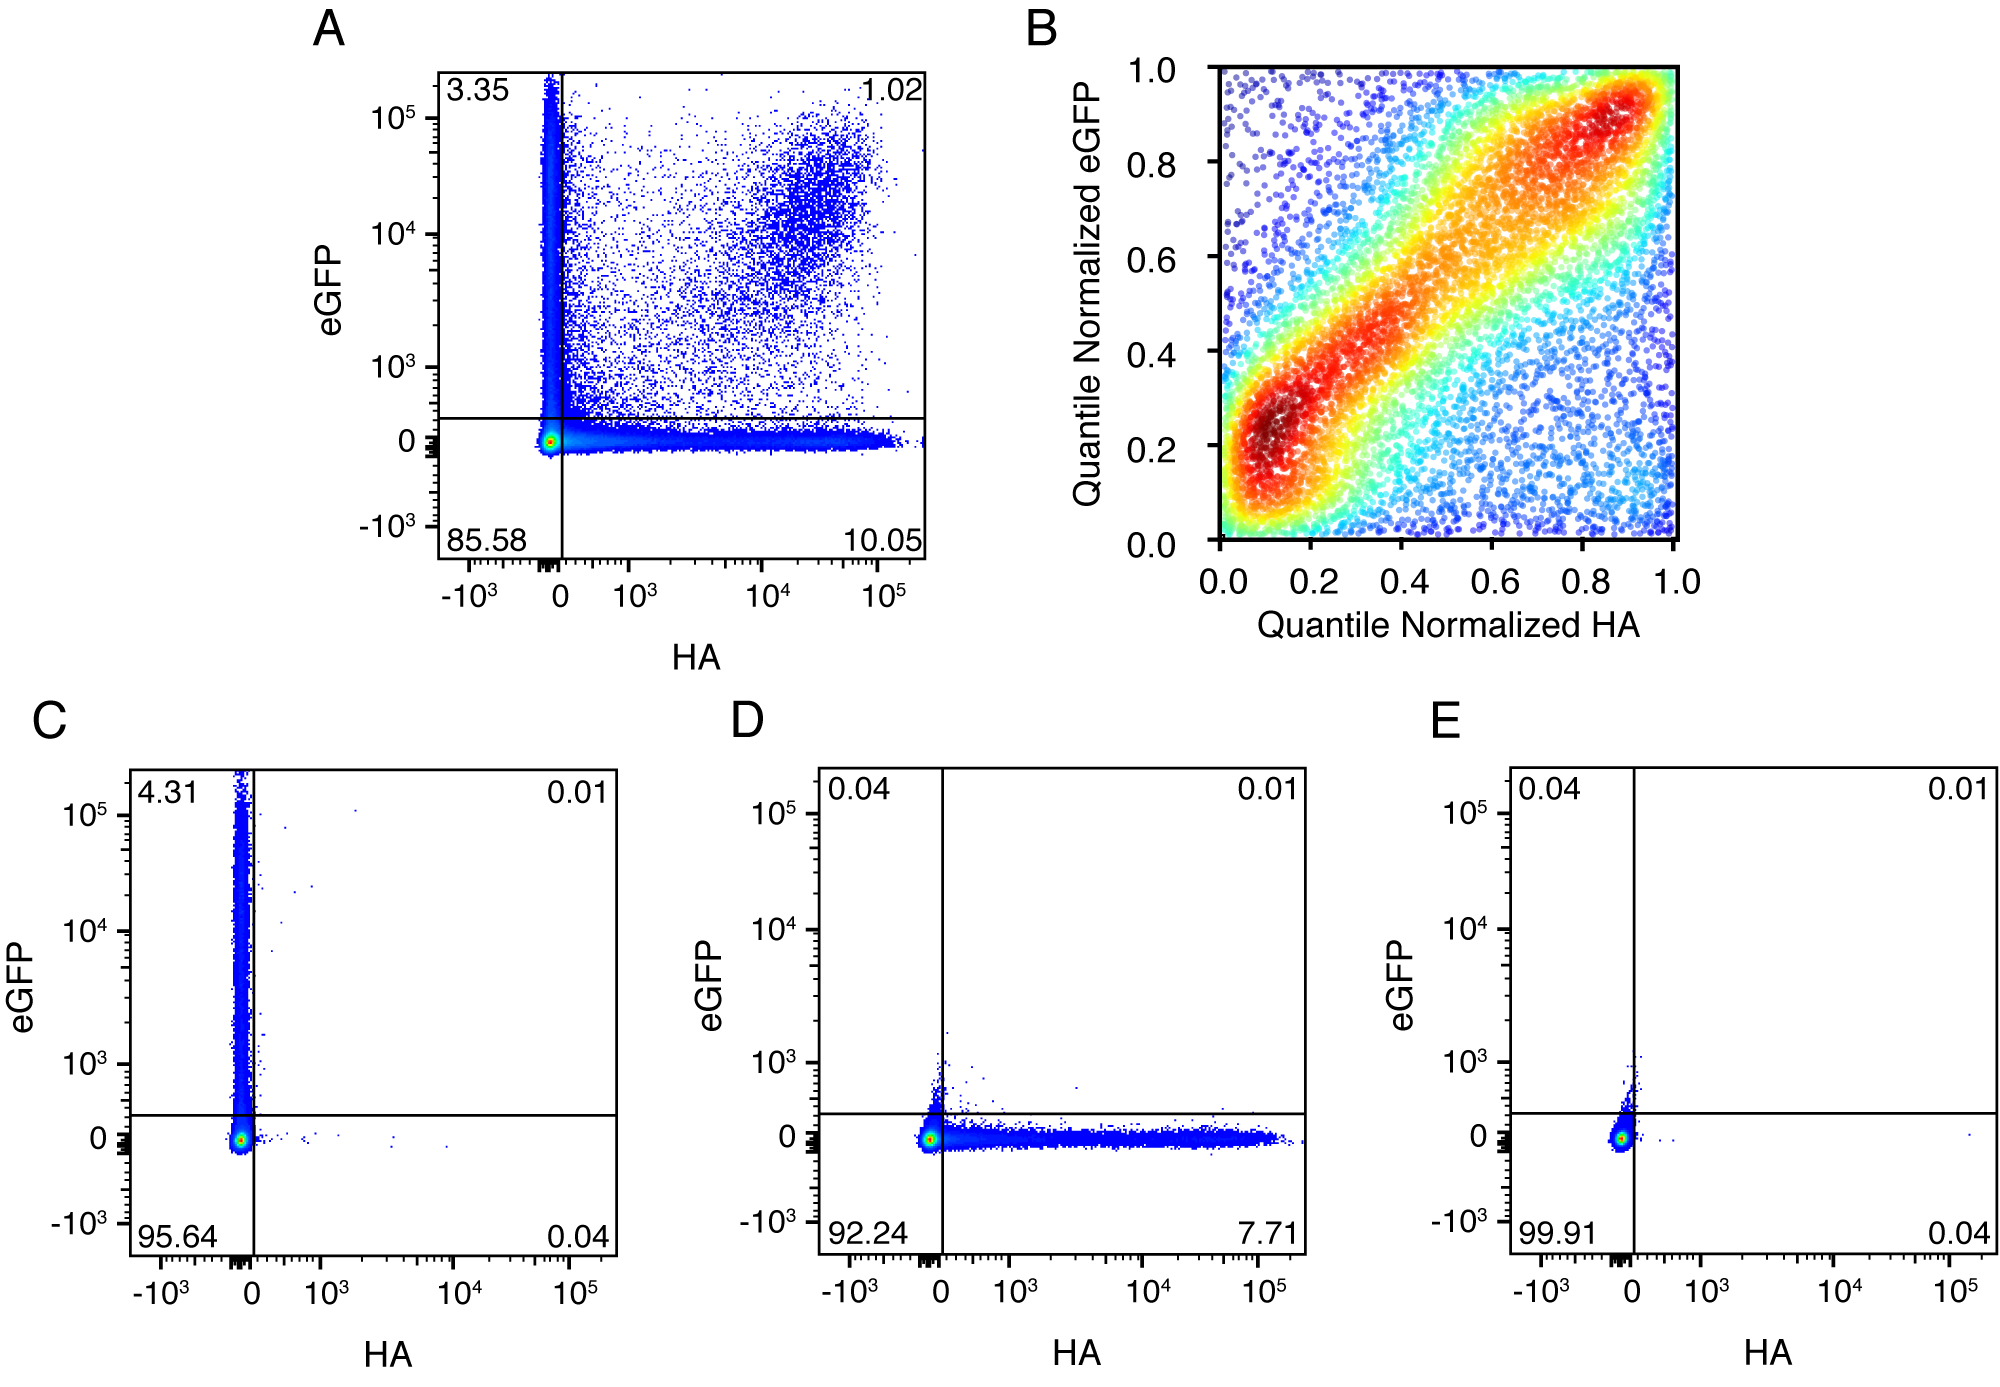
\includegraphics[width=\linewidth]{figures/Pseudovirus_flow_cytometry/coinfFlow_D02.png}}
\figdata{The raw data plotted in this figure are in \texttt{p\_co-infection.csv}.}
\end{figure}

Another observation from Figure~\ref{fig:coexpression} is that co-infected cells usually express roughly equal amounts of transcripts from each of the two viral variants.
This observation is consistent with the finding by \citet{dou2017analysis} that the temporal window for co-infection is short -- if both viral variants infect a cell at about the same time, then neither will have a headstart and so each will have a roughly equal opportunity to transcribe its genes.

To support this idea with a larger dataset albeit at lower resolution, we generated a virus in which the HA coding sequence was replaced by GFP.
We then co-infected cells with a mix of wildtype and $\Delta$HA-GFP virus and used flow cytometry to score cells for the presence of HA only (infection by wildtype virus), GFP only (infection by $\Delta$HA-GFP virus), or both (co-infection) as shown in Figure~\ref{fig:coexpression}~Figure~supplement~\ref{figsupp:flowcyto}.
As in our single-cell sequencing data, we found that expression of HA and GFP were highly correlated, indicating that co-infected cells typically expressed roughly equal amounts of transcript from each viral variant.

\subsection{Activation of the anti-viral response is rare in single infected cells.}
Because our sequencing captured all polyadenylated transcripts, we can examine whether there are prominent changes in the host-cell transcriptome in sub-populations of infected cells.
In particular, influenza virus infection can activate innate-immune sensors that lead to the transcriptional induction of type I and III interferons, and subsequently of anti-viral interferon-stimulated genes.
In bulk cells, this interferon response is one of the most prominent transcriptional signatures of influenza-virus infection.
However, activation of the interferon response is known to be stochastic and bi-modal at the level of single cells~\citep{shalek2013single,shalek2014single,bhushal2017cell}.
We therefore hypothesized that we might see two sub-populations of infected cells: one in which activation of the interferon response inhibited viral transcription, and another in which the virus was able to express high levels of its mRNA by evading or blocking this response.

\begin{figure}
\centerline{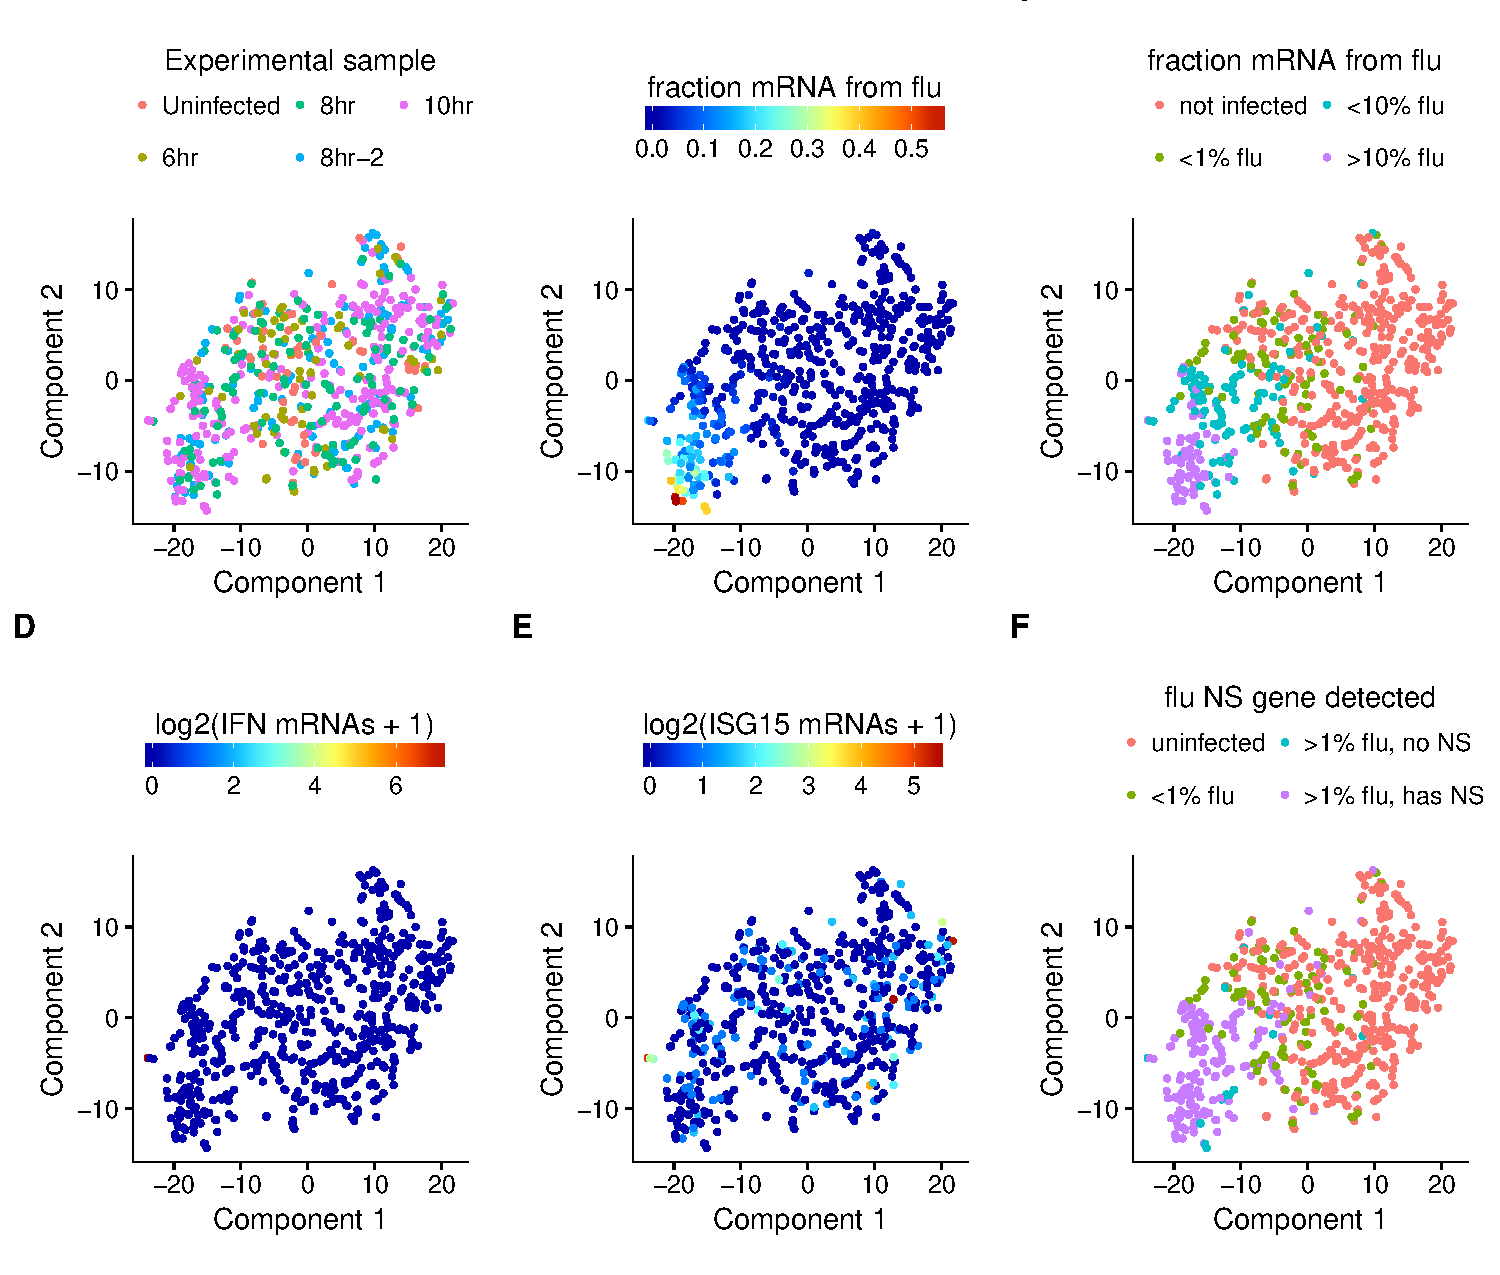
\includegraphics[width=0.8\linewidth]{figures/p_small_tsne_merge.pdf}}
\caption{\label{fig:tsne}
tSNE plots.
The layout is the same in all panels, but each panel colors the cells according to a different property.
{\bf (A), (B)}
Cells colored by the fraction of their mRNA that is viral.
{\bf (C)}
Cells colored by experimental sample.
{\bf (D)}
Cells colored by the number of type I and III interferon transcripts detected.
Only one cell has high expression of these interferons.
{\bf (E)}
Cells colored by the expression of the interferon-stimulated gene IFIT1.
{\bf (F)}
For cells with at least 1\% of their reads from influenza, are the cells expressing the viral NS protein?
The one interferon-positive cell is lacking NS, but many other cells also lack NS but do not express interferon.
}

\end{figure}

To examine whether there were distinct sub-populations among the virus-infected cells, we first used a semi-supervised t-SNE approach to cluster cells using genes that co-varied with viral infection status.
As shown in Figure~\ref{fig:tsne}A,B, this approach effectively grouped cells by the amount of viral mRNA that they expressed.
Any sample-to-sample variation was largely regressed away during the clustering, as the cells did not obviously group by time-point with the exception of the fact that the uninfected and 6-hour samples had few cells in the region of the plot corresponding to large amounts of viral mRNA (Figure~\ref{fig:tsne}C).

But to our surprise, we did not see a prominent clustering of infected cells into sub-populations as might be expected if the interferon response was strongly activated in some cells.
To investigate further, we annotated each cell by the total number of type I and III interferon transcripts observed.
Remarkably, only a single cell expressed detectable interferon (Figure~\ref{fig:tsne}D).
We also examined interferon-stimulated genes, which are induced by autocrine and paracrine interferon signaling.
Figure~\ref{fig:tsne}E shows expression of one such interferon-stimulated gene, IFIT1.
As with interferon itself, expression of IFIT1 was rare and most prominent in the single interferon-positive cell, presumably due to the higher efficiency of autocrine versus paracrine signaling.
Notably, interferon and interferon-stimulated genes were also relatively ineffective at blocking viral transcription in the single cell in which they were potently induced, since $>$10\% of the mRNA in this cell was derived from virus (Figure~\ref{fig:tsne}A,B,D,E).

We posited that the paucity of interferon activation might be due to the activity of influenza virus's major interferon antagonist, the NS1 protein.
We therefore identified cells that expressed substantial amounts of viral mRNA but lacked the NS gene (Figure~\ref{fig:tsne}F).
Consistent with the idea that NS1 is important for suppressing interferon, the one interferon-positive cell lacked detectable expression of the NS gene.
But other cells also that lacked NS expression still failed to induce a detectable interferon response, despite often having $>$10\% of their mRNA derived from virus (Figure~\ref{fig:tsne}).
Therefore, most infected cells fail to express interferon even when the virus lacks its major known interferon antagonist.
Our results are in line with other work showing that NS1-deficient influenza virus fails to deterministically induce interferon in infected cells~\citep{killip2017single}.
Therefore, single cells infected at low MOI with a relatively ``pure'' stock of influenza virus clearly activate innate-immune responses much less frequently than might be presumed from bulk studies that flood cells with viral stocks full of defective particles.

\subsection{Influenza infection is associated with the antioxidant response}

The innate immune response, often observed to be one of the most dramatic feature of influenza infection, does not appear to be a major feature of the influenza-associated host transcriptome in our single-cell data.
We therefore sought to understand whether there are additional host pathways that are significantly altered as influenza infection progresses.
Our data with respect to the NS segment suggests that presence or absence of segments might drive elements of the host response.
While of significant interest, we did not feel that we had sufficient depth to analyze such fringe elements.
We therefore restricted our analysis to only those cells in which transcripts from all eight segments were observed.
Of these cells, we furthermore normalized to host transcripts alone -- influenza is known to depress the host transcriptome and our interest lies in those cells that are more highly expressed or repressed relative to other host elements.
We then looked for genes whose expression appeared to covary with the number of influenza transcripts recovered from a cell, with a few additional caveats covered in Methods. 
With a q value threshold of 10\%, we identified a total of 45 genes.

\begin{figure}
\centerline{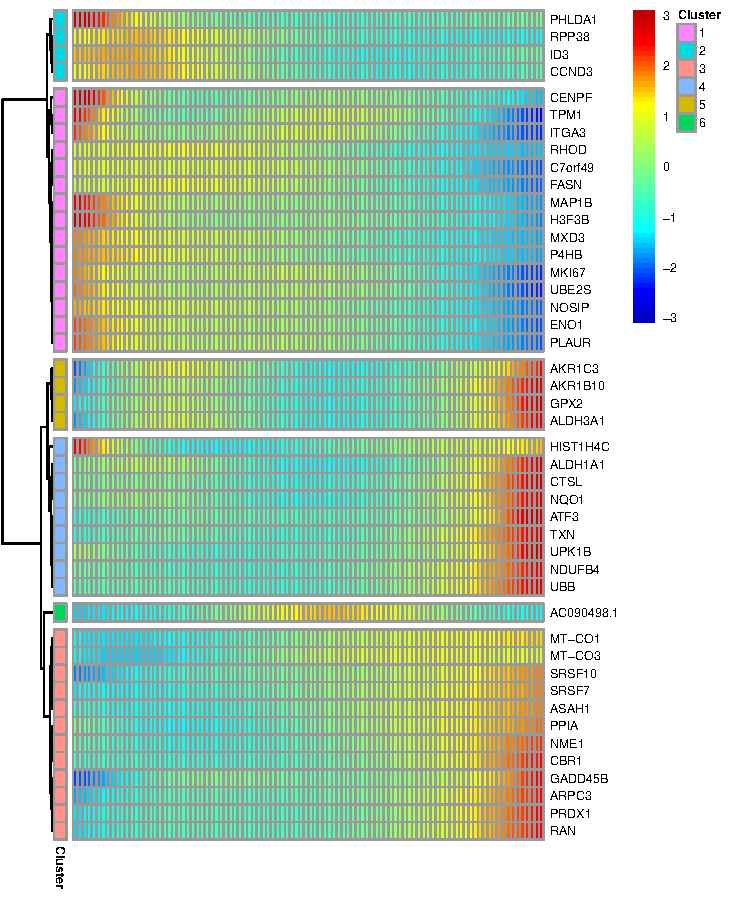
\includegraphics[width=0.7\linewidth]{figures/p_cellular_heatmap.pdf}}
\caption{\label{fig:cellulargenes}
Cellular genes that are differentially expressed with respect to the amount of influenza mRNA in individual cells infected with full influenza virus containing all eight genes.
Shown are all genes differentially expressed with $Q < 0.1$.}
\figdata{The full results of the differential expression test is in \texttt{p\_sig\_cellular\_genes.csv}.}
\figdata{The results of a gene-set analysis are in \texttt{p\_sig\_cellular\_genes.csv}.}
\figsupp[Many of the genes that exhibit co-regulation with influenza are involved in the antioxidant response. \label{figsupp:ROStable}]{
Table delineating those genes in (Figure~\ref{fig:cellulargenes}) associated with the antioxidant response.
}{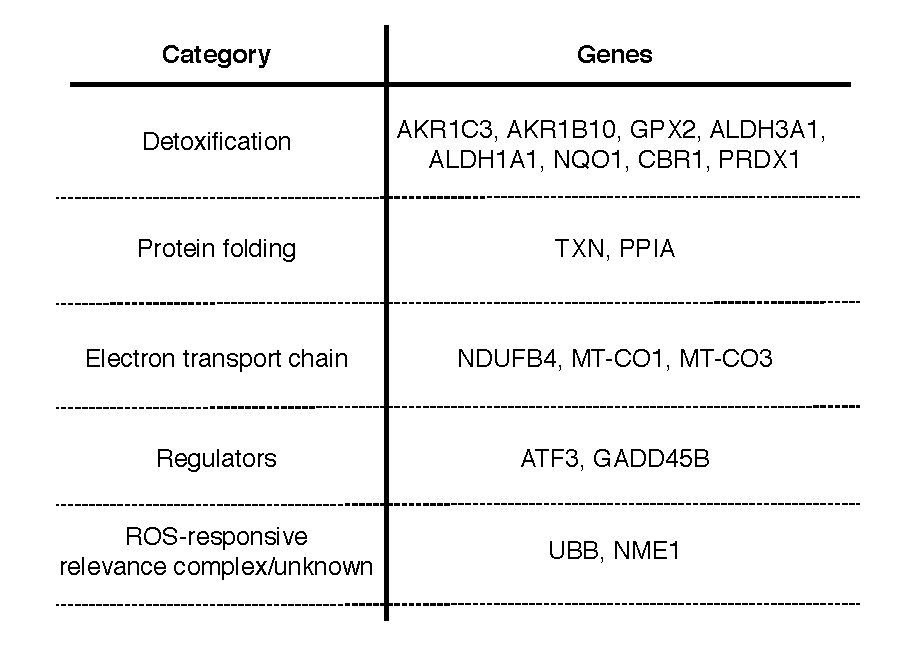
\includegraphics[width=0.7\linewidth]{figures/ROStable.pdf}}
\end{figure}

We then ordered our influenza-infected cells in pseudotime, from few influenza transcripts observed to many, and visualized expression data for these 45 genes with respect to this time course(Figure~\ref{fig:cellulargenes}).
We observe broad patterns of both repression and increased expression.
One of the most striking features of this dataset is the concomitant increase of antioxidant response genes with influenza transcript abundance.
Many of these genes are known or suspected to be regulated by the Nrf2 master regulator in response to oxidative stress, and include genes whose products are involved in detoxification of reactive oxygen species or resultant products, the management of misfolded proteins, the function of the electron transport chain, or of regulating a general stress response (Figure~supplement~\ref{figsupp:ROStable}). 
We additionally see downregulation of NOSIP, (Nitric oxide synthase interacting protein), potentially leading to elevated levels of nitric oxide. 
Transient oxidative stress has been reported in tissue culture models of influenza infection, and is thought to act in a proviral fashion through MAPK activation driving subsequent vRNP export.
We can observe here the cellular response to this stress, with multiple mechanisms driving an attempted return to homeostasis.
Curiously, the antioxidant response is thought to be largely antiviral, potentially through inhibition of MAPK activity.
Our data do not allow us to deconvolute whether the antioxidant response is driven by high levels of influenza, or vice-versa, however prior literature do suggest the former -- nevertheless we must allow that the anti-apoptotic activity of this response might be permitting cells to accumulate influenza mRNA that would otherwise have already succumbed to cell death..
We therefore suspect that the antioxidant response is the major cellular response to increasing influenza burden.
Nevertheless, its association with high levels of influenza mRNA suggests that if this response is antiviral, it must act at a level outside of transcription, or, in these experiments, it is likely engaged far too late to limit influenza in a meaningful fashion. 

\section{Discussion}

\lipsum[9]

\section{Methods and Materials}

Guidelines can be included for standard research article sections, such as this one. 

\lipsum[3]

\section{Some \LaTeX{} Examples}
\label{sec:examples}

Use section and subsection commands to organize your document. 
\LaTeX{} handles all the formatting and numbering automatically. 
Use ref and label commands for cross-references.

\subsection{Figures and Tables}


If you use the following prefixes for your \verb|\label|:
%
\begin{description}
\item[Figures] \texttt{fig:}, e.g.~\verb|\label{fig:view}|
\item[Tables] \texttt{tab:}, e.g.~\verb|\label{tab:example}|
\item[Equations] \texttt{eq:}, e.g.~\verb|\label{eq:CLT}|
\item[Boxes] \texttt{box:}, e.g.~\verb|\label{box:simple}|
\end{description}
%
you can then use the convenience commands as in \verb|\FIG{cells}|, \ to generate cross-reference \FIG{view}. 

\subsection{Citations}

LaTeX formats citations and references automatically using the bibliography records in your .bib file, which you can edit via the project menu. 
Use the \verb|\cite| command for an inline citation, like \cite{trapnell2014pseudo}, and the \verb|\citep| command for a citation in parentheses \citep{trapnell2014pseudo}. 
The LaTeX template uses a slightly-modified Vancouver bibliography style. 
If your manuscript is accepted, the eLife production team will re-format the references into the final published form. 
\emph{It is not necessary to attempt to format the reference list yourself to mirror the final published form.}


\section{Acknowledgments}

Additional information can be given in the template, such as to not include funder information in the acknowledgments section.

\nocite{*} % This command displays all refs in the bib file
\bibliography{references}


\end{document}
ommand displays all refs in the bib file
\bibliography{references}


\end{document}